\documentclass[11pt,a4paper]{report}

\usepackage{url}
\usepackage[utf8]{inputenc}
\usepackage{graphicx}
\usepackage[all]{xy}
\usepackage{amsmath}
\usepackage{amsthm}
\setlength{\marginparwidth}{2cm} 
\usepackage{todonotes}
\usepackage{array}
\usepackage{listings}
\usepackage[a4paper]{geometry}
\usepackage{csquotes}
\usepackage{amsmath,amssymb}
\usepackage{float}

\makeatletter %otherwise geometry resets everything
\Gm@restore@org
\makeatother

\setlength{\itemsep}{0cm}
\setlength{\voffset}{0cm}
\setlength{\headheight}{0cm}
\setlength{\topmargin}{0cm}
\setlength{\extrarowheight}{3pt} %for superscripts in tabular
\setlength{\arraycolsep}{4pt}
\lstset{basicstyle = \footnotesize, breaklines = true}
\usepackage[shortlabels]{enumitem}

% for the box notation
\usepackage{rotating}
\usepackage{fancyhdr}

% page number in header, right field; suppress it for float pages
\fancyfoot[R]{\iffloatpage{}{\thepage}}

% rule only in nonfloat pages
\renewcommand{\headrulewidth}{\iffloatpage{0pt}{0.4pt}}
% Actually, no rules looks better here...
\renewcommand{\headrulewidth}{0pt}

\begin{document}

\begin{titlepage}
\begin{center}
\textsc{\LARGE Bachelor thesis}\\ [0.5cm]
\textsc{ \LARGE Artificial Intelligence}\\[0.5cm]

\includegraphics[height=2cm]{Imgs/RU_Text_&_Logo.jpg}

\vspace{0.4cm}
\hrule \text{}\\[0.4cm]
\textbf{\huge Your title 
}\\[0.4cm]
\hrule
\vspace{2cm}
\begin{minipage}[t]{0.45\textwidth}
\begin{flushleft} \large
\textit{Author:}\\
Name\\
Student number
\end{flushleft}
\end{minipage}
\begin{minipage}[t]{0.45\textwidth}
\begin{flushright} \large
\textit{First supervisor:}\\
dr. A.B. LAST NAME\\
\texttt{Department}\\
\texttt{e-mail address}\\[1.3cm]
\textit{Second supervisor:}\\
dr. A.B. LAST NAME\\
\texttt{Department}\\
\texttt{e-mail address}\\[1.3cm]
\end{flushright}
\end{minipage}\\[1cm]

\includegraphics[width=4cm]{Imgs/RU_Logo.png}\\[0.5cm]
{\large \today}
\end{center}
\end{titlepage}

\begin{abstract}
The abstract of your thesis is a brief description of the research hypothesis, scientific context, motivation, and results.
The size of an abstract is usually one paragraph or one page of text.


\end{abstract}


\tableofcontents

\chapter{Introduction}\label{introduction}
The introduction of your bachelor thesis introduces the research area, the research hypothesis, and the scientific contributions of your work.
Simon Peyton Jones, a researcher at Microsoft Research, gives seven tips on how to write a great research paper which might be worth looking at
\cite{peyton_2016:HowToWriteAGreatResearchPaper}.

The following things are usually in an introduction:
\begin{itemize}
\item Describe the problem and state the research question;
\item Motivate why this problem must be solved;
\item demonstrate that a (new) solution is needed;
\item Explain the intuition behind your solution;
\item Motivate why / how your solution solves the problem (this is technical);
\item Explain briefly how it compares with related work.
\end{itemize}
%
The introduction is closed with a paragraph in which the content in the next chapters is briefly mentioned to give an overview. A guideline is one sentence per chapter. 


\chapter{Preliminaries}\label{preliminaries}
This is an optional chapter that contains knowledge that your reader needs to know in order to understand
your work. If there is not much you can also embed the preliminaries in one of the other chapters or even discard it completely. 
Your thesis audience consists of your fellow third year Artificial Intelligence bachelor students who have done the same courses as you have, but not necessarily the same electives.

\chapter{Related Work}\label{relatedwork}
Within this chapter you show that you have sufficient knowledge of the problem domain.


\chapter{Research}\label{research}
In this chapter or in these chapters you write/ show all the details that are required to \textquote {prove} your hypothesis. This should be sufficiently detailed and precise such that your fellow students are able to repeat the research and establish the same results and conclusions. 

When using large images or models you can use the appendix to improve the readability of your thesis: See the appendix \ref{appendix}. 

When you want to use a large image you might want to rotate the image, you can use boxes to use the same image in several ways:

%First create a box for the image
\newsavebox{\BoxName}
\sbox{\BoxName}{%
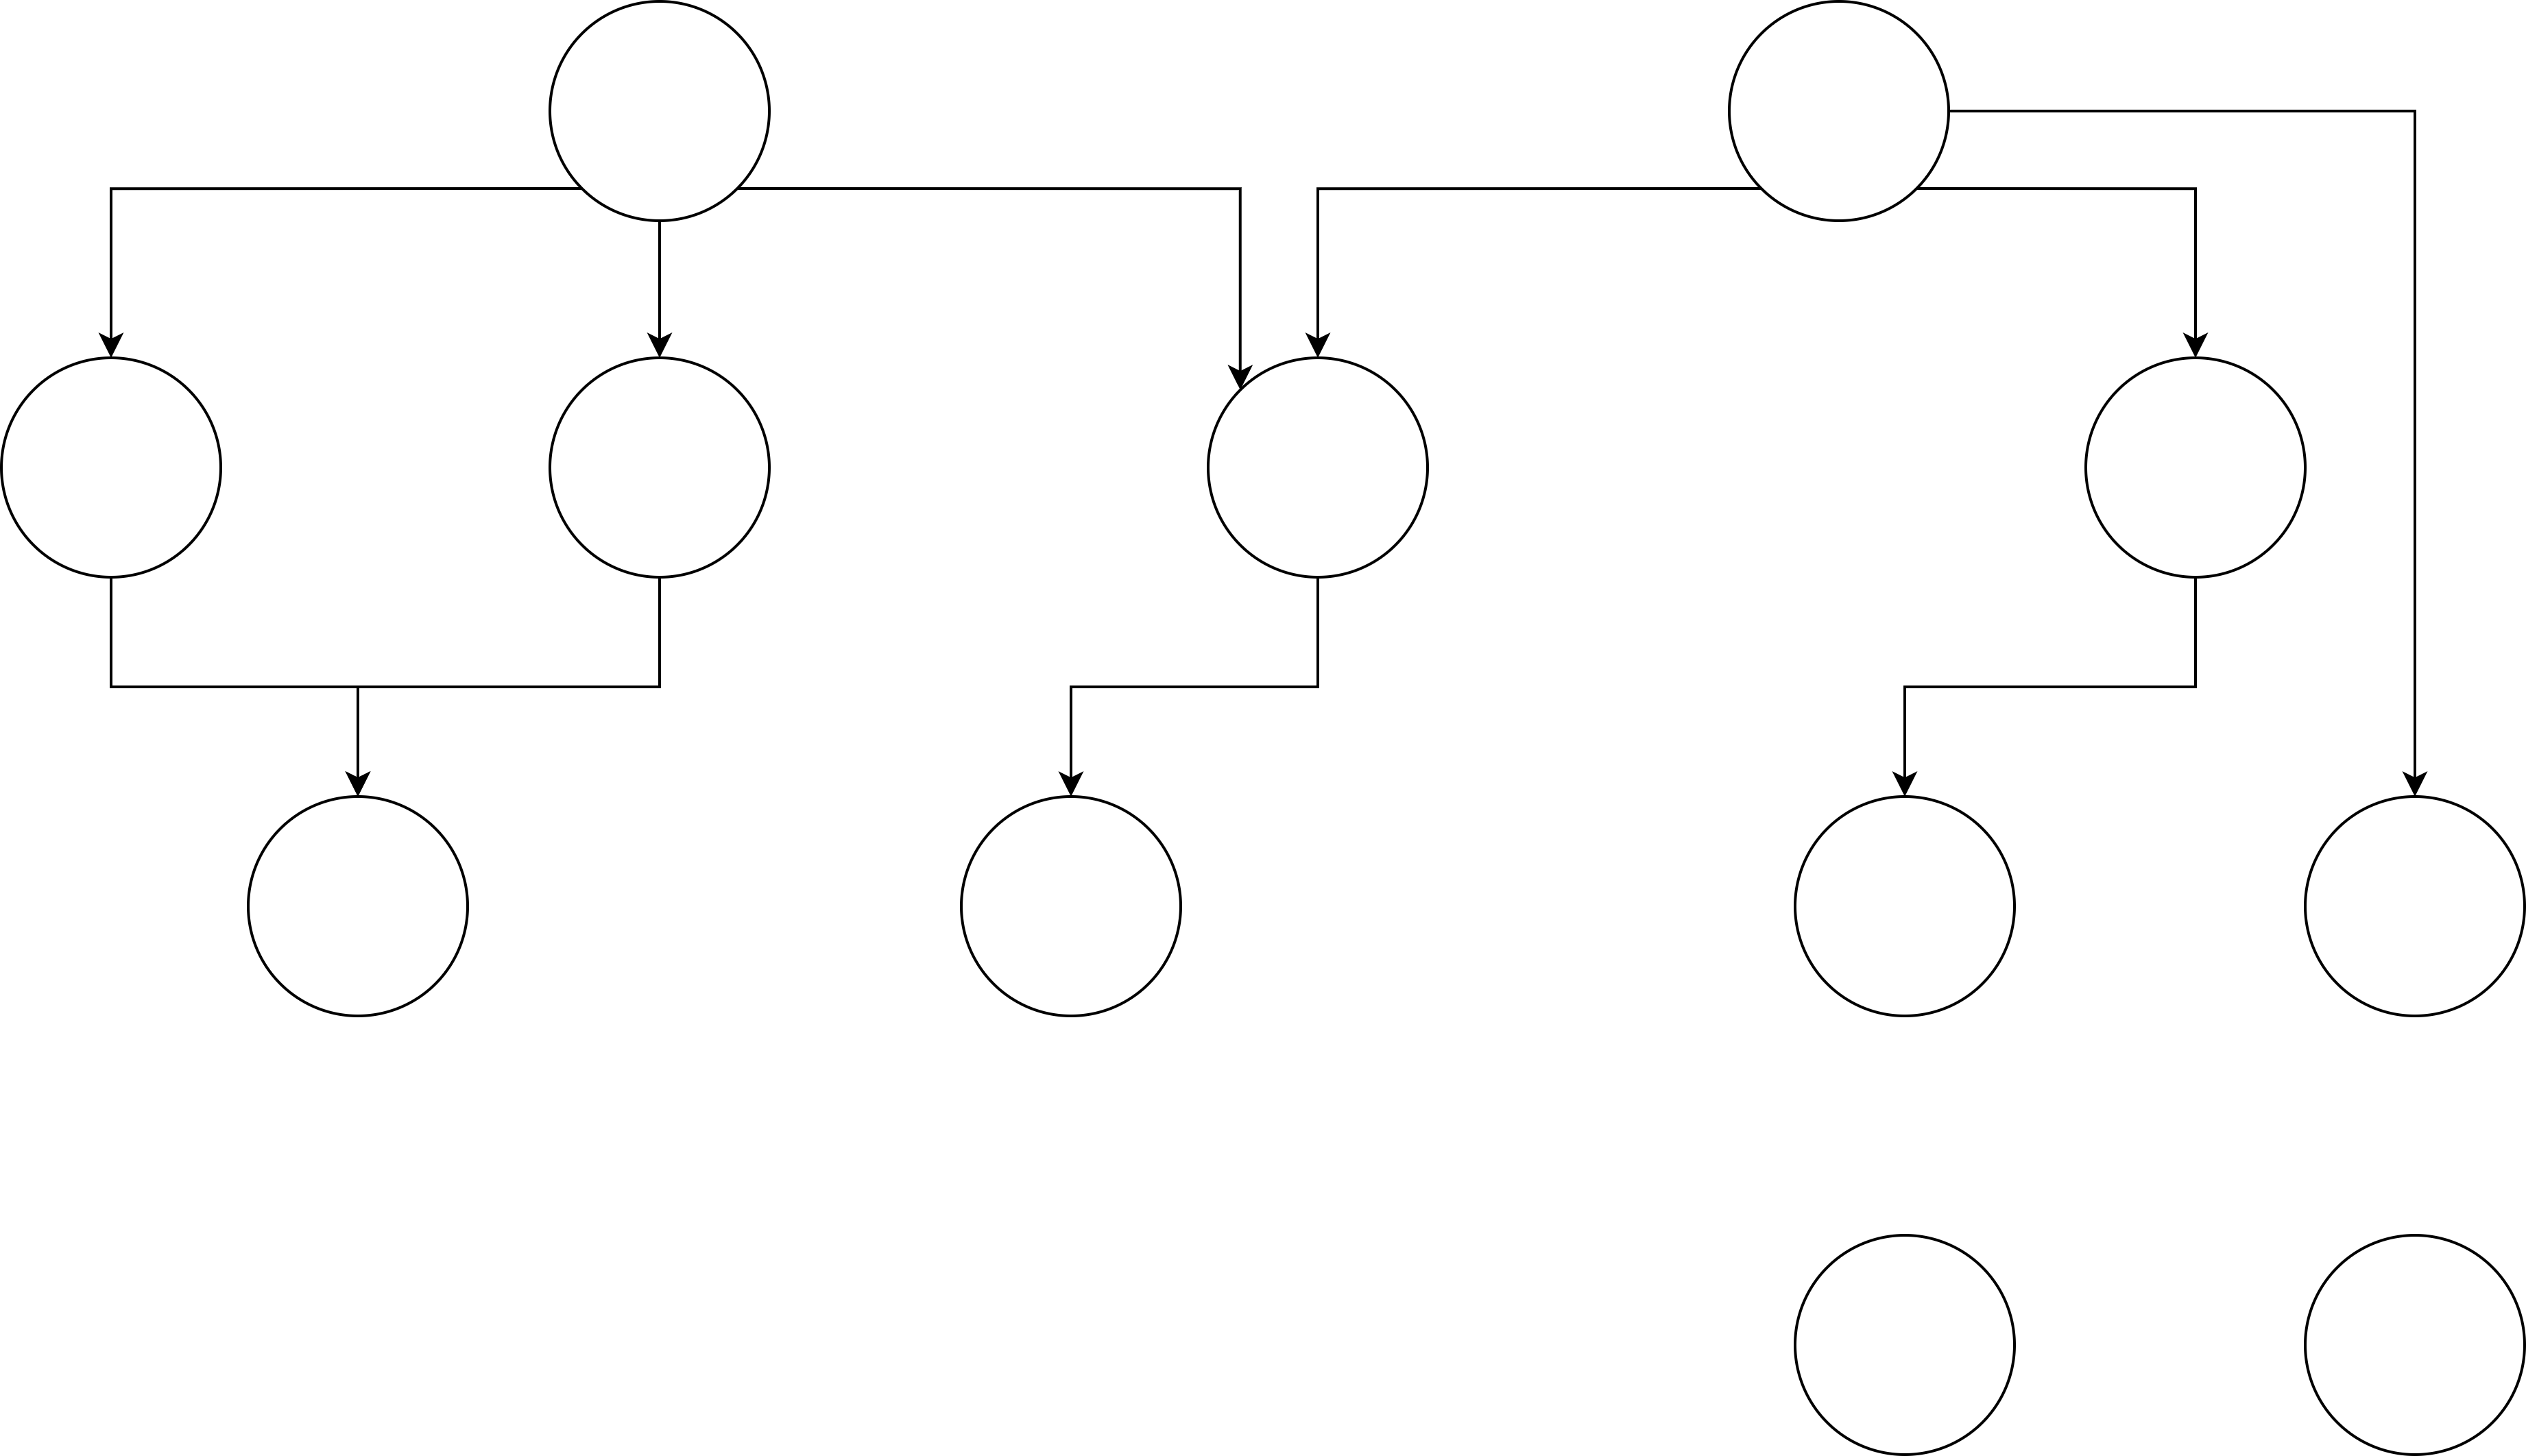
\includegraphics{Imgs/Example_model.png}
}

%The in normal text
\begin{figure}[H]
    \centerline{\resizebox{\textwidth}{!}{\usebox{\BoxName}}}
    \caption{An example image}
    \label{fig:example_image}
\end{figure}

% The rotated image (Usually put in the appendix)
\begin{sidewaysfigure}
\centerline{\resizebox{!}{0.7\textheight}{\usebox{\BoxName}}}
\caption{Rotated example image}
\label{fig:rotated_image}
\end{sidewaysfigure}
\chapter{Conclusions}\label{conclusions}
In this chapter you present all conclusions that can be drawn from the preceding chapters.
It should not introduce any new material or theories, these should have been written down earlier in the thesis. Because of this, your conclusion can be brief and to the point.





%Bibliography style is up to you 
\bibliographystyle{amsplain}
\bibliography{bibliography}

% Use when you need an appendix
\appendix
\chapter{Appendix}\label{appendix}

Appendices are optional chapters in which additional material is covered. This material is required to fully support your research, that would otherwise
clutter the presentation of your research.




\end{document}
